\documentclass[14pt,openany,a4paper,oneside]{extarticle}
\usepackage{mmap}
\usepackage{cmap}
\usepackage[T2A]{fontenc}
\usepackage[utf8]{inputenc}
\usepackage[english, russian]{babel} 
\usepackage{indentfirst}
\usepackage{graphicx}
\usepackage{color}
\usepackage{amsmath,amsfonts,amssymb,amscd,amsthm}
\usepackage[unicode, pdftex]{hyperref}
\linespread{1}
\setlength{\parindent}{1.25 cm}
\usepackage[a-1b,usecharset]{pdfx}
\usepackage[a4paper, mag=1000, left=3cm, right=2cm, top=2cm, bottom=2cm, headsep=0.7cm, footskip=1cm]{geometry}
\pagestyle{plain}
\usepackage{wrapfig}
\usepackage{mathrsfs}
\usepackage{mathtext}
\usepackage{epsf}
\usepackage{cite}
\usepackage{fancyhdr}
\usepackage{listings}
\usepackage{array}
\usepackage{ifpdf}
\usepackage{tocvsec2}
\usepackage{listings}
\usepackage{rotating}
\usepackage[normalem]{ulem} 
\usepackage{setspace}
\DeclareMathOperator{\tr}{tr}
\sloppy
\setcounter{tocdepth}{4}
\raggedbottom
\setlength{\parskip}{\medskipamount}
\renewcommand{\baselinestretch}{1} 
\usepackage{lastpage}
\makeatletter
\renewcommand{\@makecaption}[2]{
	\vspace{\abovecaptionskip}
	\sbox{\@tempboxa}{#1. #2} \ifdim \wd\@tempboxa > \hsize #1. #2\par
	\else \global\@minipagefalse \hbox \to \hsize {\hfil #1. #2\hfil}
	\fi \vspace{\belowcaptionskip}}
\makeatother
\usepackage[labelsep=period]{caption}
\usepackage{float}
\usepackage{colortbl}
\usepackage{minted}
\usepackage{dirtree}
\usepackage{float}
\captionsetup[figure]{labelfont={bf}}
\begin{document}
	\setcounter{page}{2}
	\section*{Реферат}
	\thispagestyle{empty}
	
	Объем 20 с., 4 гл., 1 табл., 5 источников, 3 прил.
	
	\textbf{Вычисление нормы одномерного интерполяционного проектора}\\
	Цель: Исследование поведения нормы интерполяционного проектора при различных конфигурациях узлов (равномерных и узлах Чебышева), а также разработка программного средства для её вычисления.\\
	Методы: Теоретический анализ свойств интерполяции, вычисление нормы по формуле Лебега, численное моделирование и визуализация результатов с использованием языка программирования Python и библиотек NumPy, Pandas, Matplotlib.\\
	Основные положения: 
	\begin{enumerate}
		\item[--] Норма интерполяционного проектора ($\|P_n\|$) характеризует устойчивость интерполяции.
		\item[--] При равномерных узлах $\|P_n\|$ растёт экспоненциально, при узлах Чебышева — логарифмически.
		\item[--] Функция Лебега ($\Lambda_n(x)$) позволяет численно находить норму, путем оценки суммы модулей базисных многочленов Лагранжа.
		\item[--] Разработана программа, позволяющая автоматизировать процесс вычислений и визуализировать зависимость нормы от числа узлов.
	\end{enumerate}
	Результаты:
	\begin{enumerate}
		\item[--] Подтверждено теоретическое преимущество узлов Чебышева для повышения устойчивости интерполяции.
		\item[--] Построены графики зависимости нормы проектора от числа узлов для обоих типов распределений.
		\item[--] Выведены практические рекомендации по выбору узлов в задачах приближённого анализа.
	\end{enumerate}
	Ключевые слова: интерполяция, норма проектора, функция Лебега, узлы Чебышева, устойчивость, Python, численные методы. 
	
	\newpage
	\def\contentsname{Содержание}
	
	\tableofcontents
	
	\newpage
	\section*{Введение}\addcontentsline{toc}{section}{Введение}
	Современные задачи анализа, моделирования и обработки информации всё чаще требуют применения численных методов, обеспечивающих высокую точность при ограниченных вычислительных ресурсах. Одним из таких методов является интерполяция — способ приближённого восстановления функции по известным значениям в конечном числе точек.
	
	Особый интерес в этом контексте представляет задача построения и анализа \textit{интерполяционного проектора} — оператора, сопоставляющего функции из заданного пространства их интерполяционные многочлены. Такая постановка позволяет не только изучать приближённые свойства интерполяции, но и оценивать устойчивость соответствующих численных алгоритмов.
	
	Одним из ключевых показателей устойчивости интерполяции является \textit{норма интерполяционного проектора}. Чем выше эта норма, тем сильнее может быть влияние ошибок или колебаний исходных данных на итоговое приближение. В частности, известное неравенство Лебега связывает ошибку интерполяции с величиной этой нормы. Таким образом, минимизация нормы проектора — важная цель при выборе узлов интерполяции. При написании курсовой
	работы использовались учебное пособие [1] и монография [2].
	
	Целью данной курсовой работы является исследование поведения нормы одномерного интерполяционного проектора при различных конфигурациях узлов: равномерных и специальных (в частности, узлов Чебышева). Особое внимание уделяется вычислительным аспектам задачи — построению алгоритма, позволяющего численно находить норму проектора по произвольному набору узлов. Программа была реализована при помощи книг [3], [4], [5]
	
	\newpage
	\section{Теоретическая часть}
	\subsection{Основные теоретические определения}
	Для понимания и решения задачи, поставленной в данной работе, необходимо сначала рассмотреть базовые понятия, лежащие в основе интерполяции и анализа интерполяционных проекторов. Эти определения и формулы обеспечивают необходимую теоретическую базу, позволяющую корректно сформулировать метод вычисления нормы интерполяционного оператора и обосновать выбор различных систем узлов.
	
	В этом разделе мы рассмотрим ключевые понятия, такие как пространство непрерывных функций $C[-1, 1]$, постановка задачи интерполяции, базисные многочлены Лагранжа, интерполяционный оператор и его норма. Особое внимание будет уделено неравенству Лебега, связывающему точность интерполяции с нормой проектора. Эти положения необходимы для обоснования численных методов, используемых в последующих разделах работы.
	
	\textbf{Пространство $C[-1,1]$}
	
	Рассмотрим пространство $C[-1,1]$, состоящее из всех непрерывных действительных функций, определённых на отрезке $[-1,1]$. Это пространство является линейным по сложению функций и умножению на число. На нём вводится равномерная норма: 
	$$\|f\|_{C[-1,1]}=\max_{x\in[-1,1]}\|f(x)\|$$
	
	С этой нормой пространство $C[-1,1]$ становится нормированным банаховым пространством, то есть полным пространством по этой норме.
	
	Практическое значение пространства $C[-1,1]$ в задачах приближения и численного анализа заключается в том, что многие функции, описывающие реальные процессы, являются непрерывными на ограниченных отрезках. Это позволяет использовать стандартные методы численного анализа, в частности, интерполяцию.
	
	\textbf{Постановка задачи интерполяции}
	
	Пусть задана функция $f \in C[-1,1]$ и набор попарно различных узлов интерполяции $x_0,x_1,\dots,x_n \in [-1,1]$. Требуется найти многочлен $p_n(x)$ степени не выше $n$, такой что: $$p_n(x_i)=f(x_i), \quad i=0,1,\dots,n.$$
	
	Такой многочлен называется интерполяционным многочленом Лагранжа, и он единственен для данного набора узлов и функции. Интерполяция позволяет аппроксимировать сложную функцию многочленом, который проще для аналитических преобразований и вычислений.
	
	Интерполяция широко применяется для:
	
	\begin{enumerate}
		\item[--] численного интегрирования и дифференцирования,
		\item[--] приближённого решения дифференциальных и интегральных уравнений,
		\item[--] построения табличных значений функций и вычислительных алгоритмов.
	\end{enumerate}
	
	\textbf{Базисные многочлены Лагранжа}
	
	Для построения интерполяционного многочлена вводятся базисные многочлены Лагранжа: $$l_i(x)=\prod^n_{\substack{m=0 \\ m \ne j}}\frac{x-x_i}{x_i-x_j},  \quad i=0,1,\dots,n.$$
	
	Эти многочлены обладают свойством: $$l_i(x_j) = \begin{cases}
		1, & \text{если $j = i$,}\\
		0, & \text{если $j \ne i$.}
	\end{cases} 
	$$
	
	Каждый многочлен $l_i(x)$ имеет степень $n$ и принимает значение 1 в узле $x_i$ и ноль во всех остальных узлах.
	
	\textbf{Интерполяционная формула Лагранжа}
	
	Интерполяционный многочлен можно записать в виде линейной комбинации базисных многочленов: $$p_n(x)=\sum^n_{i=0}f(x_i)l_i(x).$$
	
	Это выражение называется формулой Лагранжа. Оно показывает, что каждый базисный многочлен «отвечает» за одно значение функции в соответствующем узле, и сумма всех базисных многочленов образует интерполяционный многочлен.
	
	\newpage 
	
	\textbf{Понятие нормы интерполяционного проектора}
	
	Определим интерполяционный проектор $P_n:C[-1,1]\rightarrow\prod_n$, где $\prod_n$ — пространство многочленов степени не выше $n$, по правилу: $$P_nf(x)=\sum^n_{i=0}f(x_i)l_i(x).$$
	
	Этот оператор линейный и проекторный: $$P_n^2=P_n.$$
	
	Для оценки качества интерполяции вводится норма оператора $P_n$ в пространстве $C[-1,1]$ по равномерной норме: $$\|P_n\||_{C[-1,1]}=\max_{x\in[-1,1]}\|P_nf\|.$$
	
	Выражение показывает максимальное возможное усиление функции при её интерполяции. Поскольку оператор линейный, его норма равна наибольшей сумме абсолютных значений базисных многочленов: $$\|P_n\|=\max_{x\in[-1,1]}\sum_{i=0}^n|l_i(x)|=\Lambda_n.$$
	
	Величина $\Lambda_n$ называется константой Лебега.
	
	\textbf{Неравенство Лебега}
	
	Для оценки точности интерполяции используется неравенство Лебега:
	$$\|f-P_nf\|_\infty \leq (1+\Lambda_n)E_n(f),$$
	где $E_n(f)={inf}_{p\in\prod_n}\|f-p\|_\infty$ — наилучшая равномерная аппроксимация функции многочленом степени $n$.
	
	Неравенство показывает, что точность интерполяции зависит от двух факторов:
	\begin{enumerate}
		\item[--] Свойства функции $f$ — через величину $E_n(f)$.
		\item[--] Константы Лебега $\Lambda_n$ — зависящей только от расположения узлов. 
	\end{enumerate}
	
	\textbf{Мотивация к применению проекторов с мин. нормой}
	
	Константа Лебега определяет чувствительность интерполяции к погрешностям в значениях функции и ошибок округления:
	\begin{enumerate}
		\item[--] Чем больше $\Lambda_n$, тем сильнее ошибки в узловых значениях передаются на весь отрезок.
		\item[--] Малое значение $\Lambda_n$ обеспечивает устойчивость интерполяции и уменьшает глобальную погрешность.
	\end{enumerate}
	
	Например, при равномерных узлах $\Lambda_n$ растёт экспоненциально с ростом $n$, что делает интерполяцию неустойчивой. Напротив, при использовании узлов Чебышёва рост константы Лебега лишь логарифмический. Поэтому важной задачей численного анализа является подбор таких узлов, которые минимизируют $\Lambda_n$ и тем самым обеспечивают высокую точность и устойчивость интерполяции.
	
	\newpage
	\section{Практическая часть}
	\subsection{Вычисление нормы одномерного интерполяционного проектора по данному набору узлов}
	\subsubsection{Определение нормы интерполяционного проектора}
	
	Напомним, что интерполяционный проектор $P_n$ — это линейный оператор, сопоставляющий каждой функции $f\in C[-1,1]$ её интерполяционный многочлен по заданному набору узлов $x_0,x_1,\dots,x_n:$
	$$P_nf(x)=\sum^n_{i=0}f(x_i)l_i(x),$$
	где $l_i(x)$ — базисные многочлены Лагранжа.
	
	Норма оператора $P_n$ в пространстве непрерывных функций с равномерной нормой определяется как: $$\|P_n\|=\sup_{\|f\|_\infty=1}\|P_nf\|_\infty.$$
	
	Поскольку оператор линейный, достаточно рассмотреть функции $f$, принимающие значения ±1 в узлах, чтобы получить наибольшее значение $\|P_nf\|_\infty$. Это приводит к известной формуле: $$\|P_n\|=\max_{x\in[-1,1]}\Lambda_n(x),$$
	где $$\Lambda_n(x)=\sum_{i=0}^n|l_i(x)|.$$
	
	Функция $\Lambda_n(x)$ называется функцией Лебега, а её максимум на отрезке $[-1,1]$ — константой Лебега или нормой интерполяционного проектора.
	
	\subsubsection{Способ вычисления нормы по заданным узлам}
	
	Для произвольного набора узлов задача вычисления нормы проектора сводится к следующим этапам:
	\begin{enumerate}
		\item[--] Задать набор узлов $x_0,x_1,\dots,x_n.$
		\item[--] Построить базисные многочлены Лагранжа $l_i(x)$ для этих узлов: $$l_i(x)=\prod^n_{\substack{m=0 \\ m \ne j}}\frac{x-x_j}{x_i-x_j}, \quad i=0,1,\dots,n.$$
		\item[--] На отрезке $[-1,1]$ в достаточно большом числе точек (например, в 1000–5000 точках) вычислить суммы:
		$$\Lambda_n(x)=\sum^n_{i=0}|l_i(x)|.$$
		\item[--] Найти максимум функции $\Lambda_n(x)$ по всем точкам сетки: $$\Lambda_n=\max_{x\in[-1,1]}\Lambda_n(x)$$ 
	\end{enumerate}
	
	При достаточном числе точек сетки полученное значение будет очень близко к истинной норме оператора.
	\subsubsection{Нормы проекторов по равномерным узлам и узлам Чебышева}
	\textbf{Вычисление нормы для равномерных узлов}
	
	Рассмотрим интерполяцию функции на отрезке $[-1,1]$ с равномерными узлами: $$x_i=-1+\frac{2i}{n}, \quad i=0,1,\dots,n.$$
	
	Равномерное распределение узлов является самым простым вариантом, но, как показывает теория, с ростом числа узлов $n$ интерполяция на равномерной сетке становится крайне неустойчивой из-за так называемого феномена Рунге.
	
	\textbf{Теоретическая оценка нормы для равномерных узлов}
	
	Известно, что при равномерном распределении узлов константа Лебега $\Lambda_n$ растет экспоненциально: $$\frac{2^n}{8n^{3/2}} \leq \Lambda_n \leq \frac{2^n}{2}, \quad n\geq2.$$
	
	Это означает, что уже при сравнительно небольших $n$ интерполяция становится крайне чувствительной к возмущениям в исходных данных и к погрешностям вычислений.
	
	\textbf{Практический расчёт нормы для равномерных узлов}
	
	Пример расчёта (для $n=5$):
	\begin{enumerate}
		\item[--] Узлы: $x_0=-1, x_1=-0.6, x_2=-0.2, x_3=0.2, x_4=0.6, x_5=1.$
		\item[--] Вычисленная норма: $\Lambda_5 \approx 3.106$
	\end{enumerate}
	
	С увеличением $n$ значение $\Lambda_n$ быстро возрастает.
	
	\textbf{Выводы для равномерных узлов}
	
	Интерполяция на равномерных узлах допустима только для небольших $n$ и гладких функций. При больших $n$ необходимо использовать специальные распределения узлов, снижающие норму проектора.
	
	\textbf{Вычисление нормы для узлов Чебышева}
	
	Узлы Чебышева первого рода на отрезке $[-1,1]$ определяются как:
	$$x_i=\cos(\frac{2i+1}{2(n+1)}\pi), \quad i=0,1,\dots,n.$$
	
	Они расположены неравномерно, с большей плотностью у концов отрезка, что позволяет значительно снизить норму проектора и повысить устойчивость интерполяции.
	
	\textbf{Теоретическая оценка нормы для узлов Чебышева}
	
	Для узлов Чебышева первого рода известна асимптотическая оценка:
	$$\Lambda_n\leq\frac{2}{\pi}\ln(n+1)+C,$$
	где $C$ — некоторая постоянная. Это означает, что норма растёт лишь логарифмически с увеличением $n$, что в разы лучше по сравнению с экспоненциальным ростом на равномерной сетке.
	
	\textbf{Практический расчёт нормы для узлов Чебышева}
	
	Пример расчёта (для $n=5$):
	\begin{enumerate}
		\item[--] Узлы: $$x_0\approx0.97,x_1\approx0.71,x_2\approx0.26,x_3\approx-0.26,x_4\approx-0.71, x_5\approx-0.07.$$
		\item[--] Вычисленная норма: $\Lambda_5\approx2.104.$
	\end{enumerate}
	
	По сравнению с равномерными узлами результат значительно лучше.
	
	\newpage
	
	\textbf{Выводы для узлов Чебышева}
	
	На основании выполненных численных расчётов можно отметить, что нормы интерполяционных проекторов, построенных по узлам Чебышева, в проведённых примерах оказались ниже норм проекторов на равномерных узлах при одинаковом числе узлов. Это наблюдение подтверждается результатами таблицы, представленной в работе.
	
	\subsubsection{Сравнительный анализ}
	
	Для наглядности приведём сводную таблицу рассчитанных норм для равномерных и чебышёвских узлов при разных $n$:
	
	\begin{table}[h]
		\begin{center}
			\begin{tabular} {| c | c | c |}
				\hline
				$n$ & $\Lambda_{n\text{(равномерные)}}$ & $\Lambda_{n\text{(Чебышева)}}$\\
				\hline
				0 & $1$ & $1$ \\
				\hline
				1 & $1$ & $1.41$ \\
				\hline
				2 & $1.25$ & $1.67$ \\
				\hline
				3 & $1.631128$ & $1.847759$ \\
				\hline
				4 & $2.207824$ & $1.988854$ \\
				\hline
				5 & $3.106262$ & $2.104398$ \\
				\hline
				6 & $4.549336$ & $2.202215$ \\
				\hline
				7 & $6.929377$ & $2.287016$ \\
				\hline
				8 & $10.945127$ & $2.361857$ \\
				\hline
				9 & $17.847806$ & $2.428829$ \\
				\hline
				10 & $29.897759$ & $2.489430$ \\
				\hline
				11 & $51.214215$ & $2.544766$ \\
				\hline
				12 & $89.324185$ & $2.595678$ \\
				\hline
				13 & $158.084270$ & $2.642821$ \\
				\hline
				14 & $283.176228$ & $2.686715$ \\
				\hline
				15 & $512.349635$ & $2.727778$ \\
				\hline
				16 & $934.248872$ & $2.766353$ \\
				\hline
				17 & $1715.803648$ & $2.802725$ \\
				\hline
				18 & $3170.423878$ & $2.837132$ \\
				\hline
				19 & $5886.739349$ & $2.869774$ \\
				\hline
				20 & $10978.795045$ & $2.900825$ \\
				\hline
			\end{tabular}
		\end{center}
	\end{table}
	
	Вывод:
	Даже при сравнительно небольших $n$ разница в значениях норм проектора существенная. При больших $n$ преимущество узлов Чебышева становится ещё более очевидным.
	\newpage
	\subsection{Описание программы для вычисления нормы}
	
	Для численного вычисления нормы интерполяционного проектора по заданному набору узлов была разработана программа на языке Python с использованием библиотек NumPy, Pandas и Matplotlib. Программа позволяет автоматически вычислить норму оператора проекции для равномерных узлов и узлов Чебышева на отрезке $C[-1,1]$ для различного числа узлов.
	
	\subsubsection{Генерация узлов интерполяции}
	
	\textbf{Равномерные узлы} 
	
	$$x_i=-1+\frac{2i}{n}, \quad i=0,1,\dots,n$$
	\begin{minted}[fontsize=\footnotesize]{text}
		def uniform_nodes(n):
		return np.linspace(-1, 1, n + 1)
	\end{minted}
	Эта функция генерирует равномерные узлы с помощью библиотеки NumPy 
	
	\textbf{Узлы Чебышева} 
	
	$$x_i = \cos(\frac{2i+1}{2(n+1)}\pi, \quad i=0,1,\dots,n.)$$
	\begin{minted}[fontsize=\footnotesize]{text}
		def chebyshev_nodes(n):
		k = np.arange(0, n + 1)
		return np.cos((2 * k + 1) * np.pi / (2 * (n + 1)))
	\end{minted}
	Эта функция вычисляет узлы Чебышева по формуле приведенной выше.
	
	\subsubsection{Построение базисных многочленов Лагранжа}
	
	Для каждого узла $x_j$ формируется базисный многочлен $l_j(x)$ по формуле:
	$$l_j(x)=\prod^n_{\substack{m=0 \\ m \ne j}}\frac{x-x_m}{x_j-x_m}$$
	
	Эта функция выполняет данную задачу:
	\begin{minted}[fontsize=\footnotesize]{text}
		def lagrange_basis(x, nodes, j):
		xj = nodes[j]
		lj = np.ones_like(x)
		for m in range(len(nodes)):
		if m != j:
		lj *= (x - nodes[m]) / (xj - nodes[m])
		return lj
	\end{minted}
	
	\subsubsection{Вычисление функции Лебега}
	
	На равномерной сетке из 1000 точек на отрезке $[-1,1]$ рассчитывается сумма:
	
	$$\Lambda_n(x)=\sum_{j=0}^n|l_j(x)|$$
	
	Максимум этой функции на всей сетке является искомой нормой оператора:
	
	$$\|P_n\|=\max_{x\in[-1,1]}\Lambda_n(x)$$
	
	Вот таким образом эти формулы описаны в функции программы:
	\begin{minted}[fontsize=\footnotesize]{text}
		def projector_norm(nodes, x_eval):
		n = len(nodes) - 1
		L = np.zeros_like(x_eval)
		for j in range(n + 1):
		L += np.abs(lagrange_basis(x_eval, nodes, j))
		return np.max(L)
	\end{minted}
	
	\subsubsection{Интерактивный ввод параметров}
	
	При запуске программы пользователю предлагается ввести максимальное значение степени $n$, для которой необходимо рассчитать норму проектора. Это обеспечивает гибкость анализа и позволяет проводить вычисления для произвольного диапазона.
	
	\subsubsection{Сохранение и визуализация результатов}
	
	Результатом выполнения получается таблица с нормами по количеству узлов для равномерных узлов и узлов Чебышева. Все полученные значения норм сохраняются в CSV-файл.
	
	Так же программа строит график зависимостей нормы проектора от числа узлов, он позволяет наглядно сравнить поведение интерполяции при различных распределениях узлов.
	
	\newpage
	\section{Заключение}
	В данной курсовой работе было проведено подробное исследование нормы одномерного интерполяционного проектора в пространстве непрерывных функций на отрезке $C[-1,1]$ при различных распределениях интерполяционных узлов. Основное внимание было уделено сравнению поведения нормы проектора при равномерных узлах и узлах Чебышева.
	
	Теоретический анализ, подтверждённый численными экспериментами, показал, что при равномерном распределении узлов норма проектора растёт экспоненциально, что делает интерполяцию неустойчивой при больших значениях $n$. В то же время узлы Чебышева обеспечивают лишь логарифмический рост нормы, что существенно улучшает устойчивость и точность приближений.
	
	В рамках работы была разработана программа на языке Python, позволяющая автоматически вычислять норму проектора для разных типов узлов и степеней интерполяционного многочлена. Визуализация результатов подтвердила теоретические выводы и позволила наглядно сравнить поведение норм в зависимости от числа узлов.
	
	Полученные результаты подчёркивают важность правильного выбора узлов интерполяции в задачах численного анализа и аппроксимации функций. Использование узлов Чебышева является предпочтительным решением при необходимости обеспечить высокую точность и устойчивость интерполяции.
	\newpage
	
	\begin{thebibliography}{2}
		\addcontentsline{toc}{section}{Список литературы}
		
		\bibitem{1}
		Некоторые вопросы теории приближения функций / М. В. Невский, И. П. Иродова. - учеб. пособие, Яросл. гос. ун-т. Ярославль, 1999. 92 с.
		
		\bibitem{2}
		Вычислительные применения многочленов и рядов Чебышева / С. Пашковский; Пер. с польского С. Н. Киро. - Москва : Наука, 1983. - 384 с.
		
		\bibitem{3}
		Mark Lutz. Learning Python: Powerful Object-Oriented Programming / Mark Lutz. 5th edition. : O'Reilly Media, 2013. 1650 p.
		
		\bibitem{4}
		Основы работы с библиотекой NumPy / А. Н. Титов, Р. Ф. Тазиева. Минобрнауки России, Казан. нац. исслед. технол. ун-т. - Казань : Изд-во КНИТУ, 2024. - 112 с.
		
		\bibitem{5}
		Изучаем pandas / Хейдт М. пер. с англ. А. В. Груздева. -М.: ДМК Пресс, 2018. -438с.
		
	\end{thebibliography}
	\newpage
	
	\begin{flushright}Приложение А\end{flushright}
	\centerline{\textbf{Код программы}}
	\addcontentsline{toc}{section}{Приложение A}
	\begin{minted}[fontsize=\footnotesize]{text}
		syntax = "python";
		
		import numpy as np
		import pandas as pd
		import matplotlib.pyplot as plt
		
		# Генерация равномерных узлов
		def uniform_nodes(n):
		return np.linspace(-1, 1, n + 1)
		
		# Генерация узлов Чебышева
		def chebyshev_nodes(n):
		k = np.arange(0, n + 1)
		return np.cos((2 * k + 1) * np.pi / (2 * (n + 1)))
		
		# Вычисление базисного многочлена Лагранжа l_j(x)
		def lagrange_basis(x, nodes, j):
		xj = nodes[j]
		lj = np.ones_like(x)
		for m in range(len(nodes)):
		if m != j:
		lj *= (x - nodes[m]) / (xj - nodes[m])
		return lj
		
		# Норма интерполяционного проектора ||P|| = max_{x in [-1,1]} sum_j |l_j(x)|
		def projector_norm(nodes, x_eval):
		n = len(nodes) - 1
		L = np.zeros_like(x_eval)
		for j in range(n + 1):
		L += np.abs(lagrange_basis(x_eval, nodes, j))
		return np.max(L)
		
		# Главная функция вычислений
		def compute_norms(max_n):
		x_eval = np.linspace(-1, 1, 1000)
		results = []
		
		for n in range(1, max_n + 1):
		un_nodes = uniform_nodes(n)
		ch_nodes = chebyshev_nodes(n)
		norm_uniform = projector_norm(un_nodes, x_eval)
		norm_chebyshev = projector_norm(ch_nodes, x_eval)
		results.append((n, norm_uniform, norm_chebyshev))
		
		df = pd.DataFrame(results, columns=["n", "Uniform Nodes", "Chebyshev Nodes"])
		return df
		
		# Интерактивный ввод и запуск
		if __name__ == "__main__":
		try:
		user_n = int(input("Введите максимальное значение степени интерполяционного многочлена n (например, 20): "))
		if user_n <= 0:
		raise ValueError("Число должно быть положительным.")
		except ValueError as e:
		print(f"Ошибка: {e}")
		exit(1)
		
		df = compute_norms(user_n)
		print("\nРезультаты вычислений:\n")
		print(df)
		
		# Сохранение результатов
		df.to_csv("projector_norms.csv", index=False)
		
		# Построение графика
		plt.plot(df["n"], df["Uniform Nodes"], label="Равномерные узлы", marker="o")
		plt.plot(df["n"], df["Chebyshev Nodes"], label="Узлы Чебышёва", marker="x")
		plt.xlabel("n (степень интерполяционного многочлена)")
		plt.ylabel("Норма проектора")
		plt.title("Сравнение норм интерполяционных проекторов")
		plt.legend()
		plt.grid(True)
		plt.show()
		
	\end{minted}
	\newpage
	
	\begin{flushright}Приложение Б\end{flushright}
	\centerline{\textbf{Вывод программы}}
	\addcontentsline{toc}{section}{Приложение Б}
	
	\begin{minted}[fontsize=\footnotesize]{text}
		n  Uniform Nodes  Chebyshev Nodes
		1       1.000000         1.414214
		2       1.250000         1.666667
		3       1.631128         1.847759
		4       2.207824         1.988854
		5       3.106262         2.104398
		6       4.549336         2.202215
		7       6.929377         2.287016
		8      10.945127         2.361857
		9      17.847806         2.428829
		10      29.897759         2.489430
		11      51.214215         2.544766
		12      89.324185         2.595678
		13     158.084270         2.642821
		14     283.176228         2.686715
		15     512.349635         2.727778
		16     934.248872         2.766353
		17    1715.803648         2.802725
		18    3170.423878         2.837132
		19    5886.739349         2.869774
		20   10978.795045         2.900825        
	\end{minted}
	
	\newpage
	
	\begin{flushright}Приложение В\end{flushright}
	\centerline{\textbf{График}}
	\addcontentsline{toc}{section}{Приложение В}
	
	\begin{center}
		\rotatebox{270}{%
			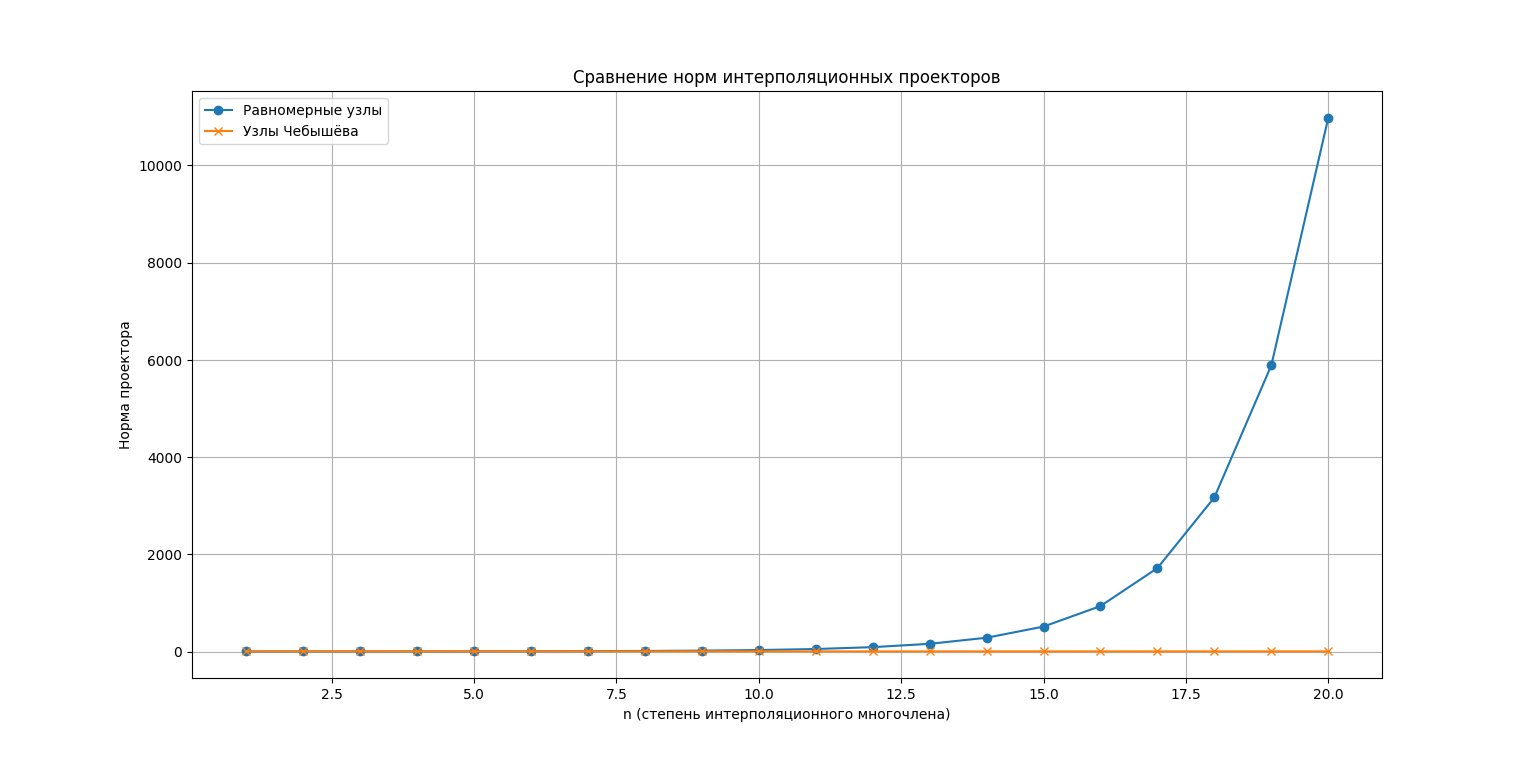
\includegraphics[height=0.72\textwidth]{projector_norms_plot.png}
		}
	\end{center}
\end{document}